\section{Equivalence of SD and ABS implementation}
After having shown that both the SD and ABS approaches are equivalent by visually comparing the dynamics of Figure \ref{fig:sir_sd_dynamics} to the ones of Figure \ref{fig:sir_10000_01dt}, we ask the question whether we can also show the equivalence of both approaches from their implementation.
First we need to show that the SD implementation is correct as in \textit{is an implementation of the mathematical definition} as it is the foundation upon we build our equivalence.

\subsection{Correctness of SD implementation}
The mathematical formulas for susceptible, infected an recovered stocks with the infection- and recover-rates are directly translated into the SD implementation as seen in Appendix \ref{app:sd_code}. We can thus assume that the translation from the mathematical definition to Haskell code is correct as it \textit{is} exactly the same. This leaves us with the question how the values of the stocks and flows are distributed between each other. When solving the mathematical equations numerically, one is dividing time into infinitely small intervals and calculates the new value of each formula at each time-interval at the same time: the values update all at the same time.
The same needs to happen in our SD implementation which is indeed the case: \textit{runSD} as seen in line 127 uses \textit{simulateTime} behind the scenes with the \textit{parallel} update-strategy which uses a \textit{map} to iterate over all agents. This implies by definition of map that all stocks and flows, which are in fact agents, update virtually at the same time. Due to pureness of runSD we can rule out side-effects which could only occur when running in the IO Monad or using unsafePerformIO \footnote{Again we use unsafePerformIO in initializing the previously mentioned agent-id generator but it is never used within the runSD implementation or any of the stocks and flows.}. 
It is clear now that the values update at the same time and calculate the correct values as defined in the mathematical formulas. The distribution of the values happens by using absolute stock- and flow-ids and it is easy to check that the ids used in \textit{flowInFrom/flowOutTo} and \textit{stockInFrom/stockOutTo} build the correct connections as seen in the Stock-And-Flow diagram in Figure \ref{fig:sir_sd_stockflow_diagramm}.
This leaves us with the implementation of \textit{integral}. Theoretically we arrive at the correct mathematical solution if we use infinitely small $\Delta t$ but this is of course impossible using a computer. When looking at the implementation of \textit{integral} it becomes apparent that it uses the rectangle-rule. TODO: need more details and look a bit into theory of numerically solving integral (e.g. classic newton, or runge-kutta). The rectangle rule needs small $\Delta t$ for sufficient accuracy as we have shown in Figure \ref{fig:sd_plots}.
For our reference dynamics in Figure \ref{fig:sir_sd_dynamics} we used $\Delta t = 0.001$, which computes 150,000 steps. When comparing it with dynamics as seen in Figure \ref{fig:sd_anylogic} generated by the professional software package AnyLogic Personal Learning Edition 8.1.0 we can safely say that a $\Delta t = 0.001$ is sufficiently small to generate matching accuracy.

\begin{figure}
	\centering
	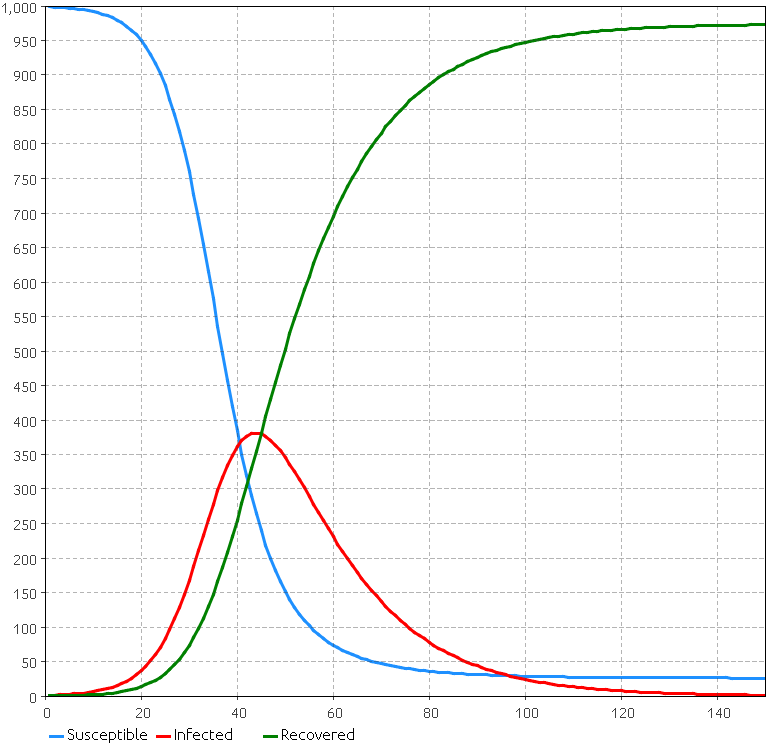
\includegraphics[width=.4\textwidth, angle=0]{./../shared/fig/anylogic/SIR_SD_DYNAMICS_ANYLOGIC.png}
	\caption{Dynamics of the SIR model using the SD approach generated with AnyLogic Personal Learning Edition 8.1.0. Population Size $N$ = 1,000, contact rate $\beta =  \frac{1}{5}$, infection probability $\gamma = 0.05$, illness duration $\delta = 15$ with initially 1 infected agent. Simulation run for 150 time-steps.}
	\label{fig:sd_anylogic}
\end{figure}

\subsection{Correctness of ABS implementation}
The question is now what \textit{correctness} of an ABS implementation means. This is indeed a very non-trivial problem and is highly dependent on the model. In our case of the agent-based SIR implementation we define correctness to mean \textit{qualitatively approximating the SD dynamics}. This means that to show that our ABS implementation is correct, we need to show that it is equivalent to the SD implementation. TODO: this is a bit short, maybe we can say more about this. need to read a few papers and get better understanding on this topic

Also we ask the question: why is it that the susceptible agents must make the contact and the infected only replying? can't just the infected agents make contact thus saving a round-trip? also why are not both making contact? When comparing the two contact-policies as seem in Figure \ref{fig:sir_abs_correctness_contactpolicies}, it is clear that both don't match neither the SD dynamics of Figure \ref{fig:sir_sd_dynamics} and ABM dynamics of Figure \ref{fig:sir_10000_01dt}.

\begin{figure*}
\begin{center}

	\begin{tabular}{c c}
		\begin{subfigure}[b]{0.5\textwidth}
			\centering
			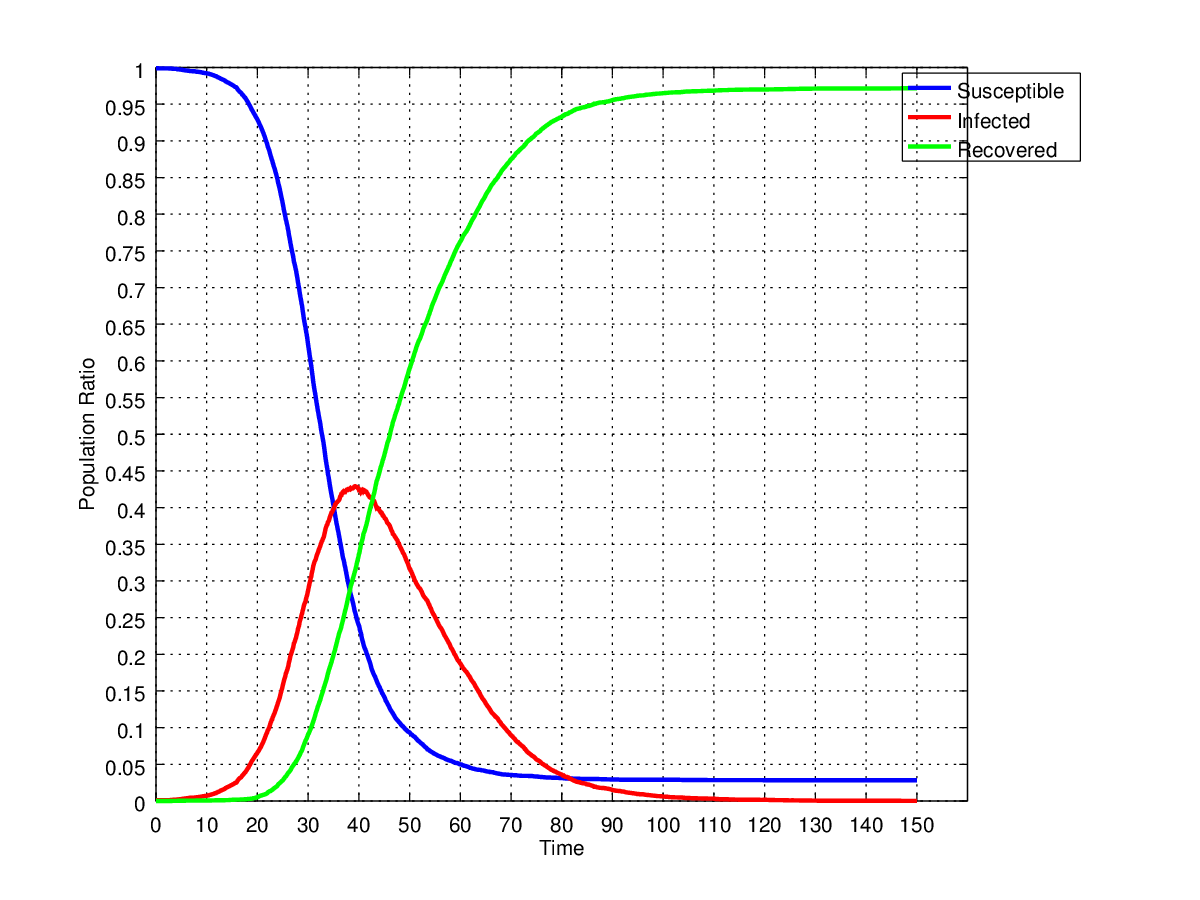
\includegraphics[width=1\textwidth, angle=0]{./../shared/fig/frabs/INFECTED_CONTACT_ONLY_SIR_10000agents_150t_01dt_parallel.png}
			\caption{Infected agents make contact.}
			\label{fig:sir_abs_correctness_contact_infected}
		\end{subfigure}
    	&
		\begin{subfigure}[b]{0.5\textwidth}
			\centering
			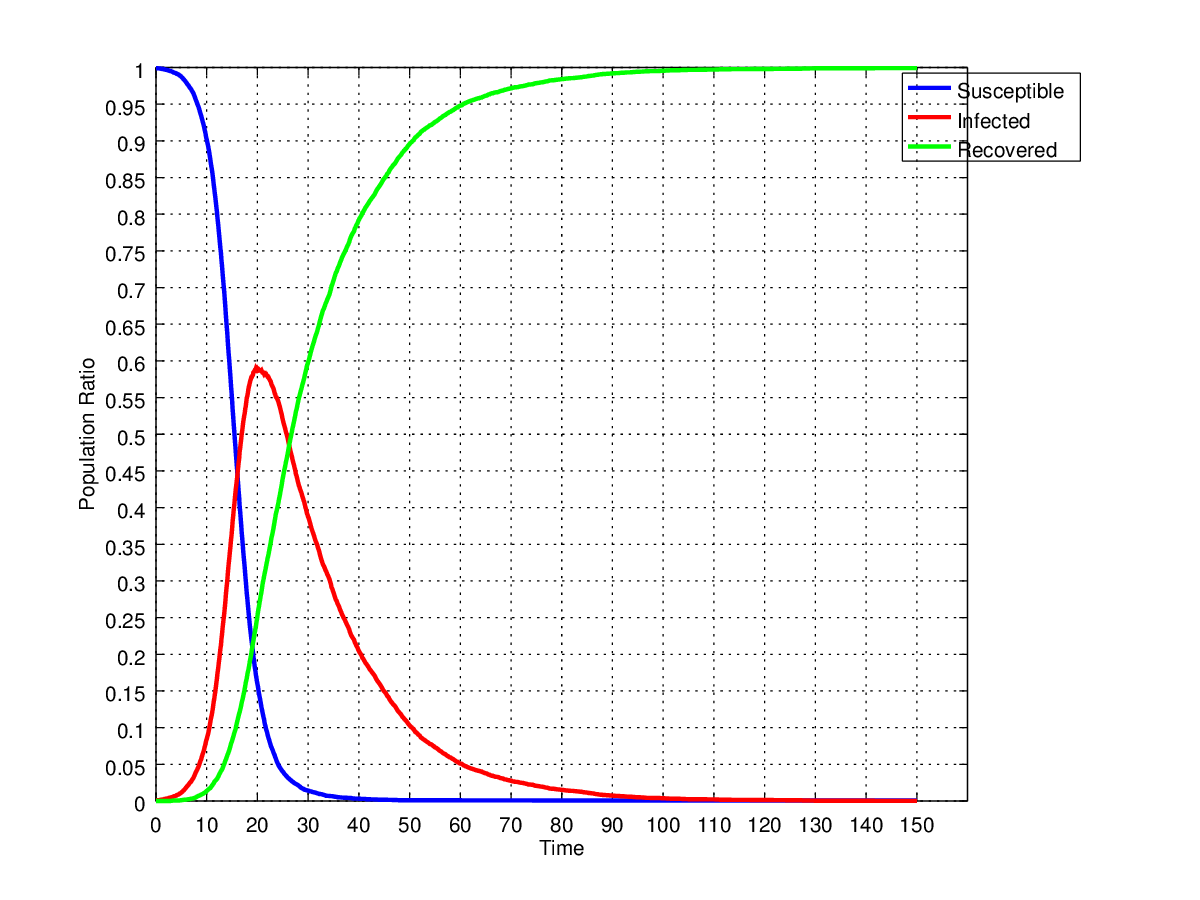
\includegraphics[width=1\textwidth, angle=0]{./../shared/fig/frabs/INFECTED_AND_SUSCEPTIBLE_CONTACT_SIR_10000agents_150t_01dt_parallel.png}
			\caption{Susceptible and Infected agents make contact.}
			\label{fig:sir_abs_correctness_contact_both}
		\end{subfigure}
	\end{tabular}
	
	\caption{Dynamics of different contact policies. Using same model parameters as in Figure \ref{fig:sir_10000_01dt}.} 
	\label{fig:sir_abs_correctness_contactpolicies}
\end{center}
\end{figure*}

\subsection{Equivalence}
TODO: need to think about this very deeply, but basically it is all about probabilities which increase with number of messages which increase with number of infected. we need somehow to match the number of messages a susceptible receives to the stocks and flows formulas
TODO: can we show why the infected themselves do not (and must not) make contact and only reply to incoming contacts?